\documentclass[hyperref={pdfpagelabels=false}]{beamer}
% Die Hyperref Option hyperref={pdfpagelabels=false} verhindert die Warnung:
% Package hyperref Warning: Option `pdfpagelabels' is turned off
% (hyperref)                because \thepage is undefined. 
% Hyperref stopped early 
%
% 
% Deutsche Spracheinstellungen
\usepackage[ngerman,german]{babel, varioref}
\usepackage[T1]{fontenc}
\usepackage[utf8]{inputenc}

%\usepackage{marvosym}

\usepackage{amsfonts}
\usepackage{amssymb}
\usepackage{amsmath}
\usepackage{amscd}
\usepackage{amstext}
\usepackage{float}
\usepackage{caption}
\usepackage{wrapfig}
\usepackage{setspace}
%\usepackage[onehalfspacing]{setspace}
\usepackage{threeparttable}
% \usepackage{footnote}
% \usepackage{feynmf}
\usepackage{bbm}
\usepackage{slashed}
\usepackage{textcomp}
\usepackage{multirow}
\usepackage{courier}
\usepackage{listings}
\usepackage{color}
%\usepackage{minipage}
 
 \definecolor{middlegray}{rgb}{0.5,0.5,0.5}
 \definecolor{lightgray}{rgb}{0.8,0.8,0.8}
 \definecolor{orange}{rgb}{0.8,0.3,0.3}
 \definecolor{yac}{rgb}{0.6,0.6,0.1}
 \definecolor{puple}{rgb}{0.62,0.12,0.94}
 \lstset{language=Python,
                basicstyle=\ttfamily,
                keywordstyle=\color{red}\ttfamily,
                stringstyle=\color{magenta}\ttfamily,
                commentstyle=\color{blue}\ttfamily,
                morecomment=[l][\color{blue}]{\#},
		%stepnumber=1,
		%numberstyle=\color{magenta}\ttfamily,
		%    numbers=left,
		%    numberstyle={},
		%    numberblanklines=false,
		%    stepnumber=1,
		%    numbersep=10pt,
		    xleftmargin=15pt,
 		moredelim=[is][\color{purple}]{|}{|}
}

\newfloat{formel}{htbp}{for}
\floatname{formel}{Formel}

% \onehalfspacing
%\setstretch {1.433}

\usepackage{longtable}

%\usepackage{bibgerm}

\usepackage{footnpag}

\usepackage{ifthen}                 %%% package for conditionals in TeX
\usepackage[amssymb]{SIunits}
%Fr textumflossene Bilder und Tablellen
%\usepackage{floatflt} - veraltet

%Fr Testzwecke aktivieren, zeigt labels und refs im Text an.
%\usepackage{showkeys}

% Abstand zwischen zwei Abs�zen nach DIN (1,5 Zeilen)
% \setlength{\parskip}{1.5ex}

% Einrckung am Anfang eines neuen Absatzes nach DIN (keine)
%\setlength{\parindent}{0pt}

% R�der definieren
% \setlength{\oddsidemargin}{0.3cm}
% \setlength{\textwidth}{15.6cm}

% bessere Bildunterschriften
%\usepackage[center]{caption2}


% Probleml�ungen beim Umgang mit Gleitumgebungen
\usepackage{float}

% Nummeriert bis zur Strukturstufe 3 (also <section>, <subsection> und <subsubsection>)
%\setcounter{secnumdepth}{3}

% Fhrt das Inhaltsverzeichnis bis zur Strukturstufe 3
%\setcounter{tocdepth}{3}

\usepackage{exscale}

\newenvironment{dsm} {\begin{displaymath}} {\end{displaymath}}
\newenvironment{vars} {\begin{center}\scriptsize} {\normalsize \end{center}}


\newcommand {\en} {\varepsilon_0}               % Epsilon-Null aus der Elektrodynamik
\newcommand {\lap} {\; \mathbf{\Delta}}         % Laplace-Operator
\newcommand {\R} { \mathbb{R} }                 % Menge der reellen Zahlen
\newcommand {\e} { \ \mathbf{e} }               % Eulersche Zahl
\renewcommand {\i} { \mathbf{i} }               % komplexe Zahl i
\newcommand {\N} { \mathbb{N} }                 % Menge der nat. Zahlen
\newcommand {\C} { \mathbb{C} }                 % Menge der kompl. Zahlen
\newcommand {\Z} { \mathbb{Z} }                 % Menge der kompl. Zahlen
\newcommand {\limi}[1]{\lim_{#1 \rightarrow \infty}} % Limes unendlich
\newcommand {\sumi}[1]{\sum_{#1=0}^\infty}
\newcommand {\rot} {\; \mathrm{rot} \,}         % Rotation
\newcommand {\grad} {\; \mathrm{grad} \,}       % Gradient
\newcommand {\dive} {\; \mathrm{div} \,}        % Divergenz
\newcommand {\dx} {\; \mathrm{d} }              % Differential d
\newcommand {\cotanh} {\; \mathrm{cotanh} \,}   %Cotangenshyperbolicus
\newcommand {\asinh} {\; \mathrm{areasinh} \,}  %Area-Sinus-Hyp.
\newcommand {\acosh} {\; \mathrm{areacosh} \,}  %Area-Cosinus-H.
\newcommand {\atanh} {\; \mathrm{areatanh} \,}  %Area Tangens-H.
\newcommand {\acoth} {\; \mathrm{areacoth} \,}  % Area-cotangens
\newcommand {\Sp} {\; \mathrm{Sp} \,}
\newcommand {\mbe} {\stackrel{\text{!}}{=}}     %Must Be Equal
% \newcommand{\qed} { \hfill $\square$\\}
\newcommand{\midtilde}{\raisebox{-0,25\baselineskip}{\textasciitilde}}
\renewcommand{\i} {\imath}
\def\captionsngerman{\def\figurename{\textbf{Abb.}}}

%%%%%%%%%%%%%%%%%%%%%%%%%%%%%%%%%%%%%%%%%%%%%%%%%%%%%%%%%%%%%%%%%%%%%%%%%%%%
% SWITCH FOR PDFLATEX or LATEX
%%%%%%%%%%%%%%%%%%%%%%%%%%%%%%%%%%%%%%%%%%%%%%%%%%%%%%%%%%%%%%%%%%%%%%%%%%%%
%%%
\ifx\pdfoutput\undefined %%%%%%%%%%%%%%%%%%%%%%%%%%%%%%%%%%%%%%%%% LATEX %%%
%%%
\usepackage[dvips]{graphicx}       %%% graphics for dvips
\DeclareGraphicsExtensions{.eps,.ps}   %%% standard extension for included graphics
\usepackage[ps2pdf]{thumbpdf}      %%% thumbnails for ps2pdf
\usepackage[ps2pdf,                %%% hyper-references for ps2pdf
bookmarks=true,%                   %%% generate bookmarks ...
bookmarksnumbered=true,%           %%% ... with numbers
hypertexnames=false,%              %%% needed for correct links to figures !!!
breaklinks=true,%                  %%% breaks lines, but links are very small
linkbordercolor={0 0 1},%          %%% blue frames around links
pdfborder={0 0 112.0}]{hyperref}%  %%% border-width of frames
%                                      will be multiplied with 0.009 by ps2pdf
%
\hypersetup{ pdfauthor   = {Hannes Franke; Julius Tilly},
pdftitle    = {V301 Innenwiderstand und Leistungsanpassung}, pdfsubject  = {Protokoll FP}, pdfkeywords = {V301, Innenwiderstand, Leistungsanpassung},
pdfcreator  = {LaTeX with hyperref package}, pdfproducer = {dvips
+ ps2pdf} }
%%%
\else %%%%%%%%%%%%%%%%%%%%%%%%%%%%%%%%%%%%%%%%%%%%%%%%%%%%%%%%%% PDFLATEX %%%
%%%
\usepackage[pdftex]{graphicx}      %%% graphics for pdfLaTeX
% \DeclareGraphicsExtensions{.pdf}   %%% standard extension for included graphics
% \usepackage[pdftex]{thumbpdf}      %%% thumbnails for pdflatex
\usepackage[pdftex,                %%% hyper-references for pdflatex
bookmarks=true,%                   %%% generate bookmarks ...
bookmarksnumbered=true,%           %%% ... with numbers
hypertexnames=false,%              %%% needed for correct links to figures !!!
breaklinks=true,%                  %%% break links if exceeding a single line
linkbordercolor={0 0 1},
linktocpage]{hyperref} %%% blue frames around links
%                                  %%% pdfborder={0 0 1} is the default
\hypersetup{
pdftitle    = {V301 Innenwiderstand und Leistungsanpassung}, 
pdfsubject  = {Protokoll AP}, 
pdfkeywords = {V301, Innenwiderstand, Leistungsanpassung},
pdfsubject  = {Protokoll AP},
pdfkeywords = {V301, Innenwiderstand, Leistungsanpassung}}
%                                  %%% pdfcreator, pdfproducer,
%                                      and CreationDate are automatically set
%                                      by pdflatex !!!
\pdfadjustspacing=1                %%% force LaTeX-like character spacing
\usepackage{epstopdf}
%
\fi %%%%%%%%%%%%%%%%%%%%%%%%%%%%%%%%%%%%%%%%%%%%%%%%%%% END OF CONDITION %%%
%%%%%%%%%%%%%%%%%%%%%%%%%%%%%%%%%%%%%%%%%%%%%%%%%%%%%%%%%%%%%%%%%%%%%%%%%%%%
% seitliche Tabellen und Abbildungen
%\usepackage{rotating}
\usepackage{ae}
\usepackage{
  array,
  booktabs,
  dcolumn
}
\makeatletter 
  \renewenvironment{figure}[1][] {% 
    \ifthenelse{\equal{#1}{}}{% 
      \@float{figure} 
    }{% 
      \@float{figure}[#1]% 
    }% 
    \centering 
  }{% 
    \end@float 
  } 
  \makeatother 


  \makeatletter 
  \renewenvironment{table}[1][] {% 
    \ifthenelse{\equal{#1}{}}{% 
      \@float{table} 
    }{% 
      \@float{table}[#1]% 
    }% 
    \centering 
  }{% 
    \end@float 
  } 
  \makeatother 
%\usepackage{listings}
%\lstloadlanguages{[Visual]Basic}
%\allowdisplaybreaks[1]
%\usepackage{hycap}
%\usepackage{fancyunits}

 %\usepackage{german}
\usepackage{graphicx}
%\usepackage[latin1]{inputenc}
\usepackage{Tex/nicehead}
\usepackage{epsfig}
\usepackage{amssymb}
\usepackage{amsmath}
\usepackage{tabularx}
\usepackage{calc}
\usepackage[vflt]{floatflt}
\usepackage{units}
\usepackage{upgreek}
%\usepackage[pdfborder={0 0 0}, hypertexnames=false]{hyperref}
\usepackage[official]{eurosym}

% Seitenstil
\pagestyle{emheadings}

% Breite des Textblocks und der Raender
\setlength{\evensidemargin}{0mm}
\setlength{\oddsidemargin}{13mm}
\setlength{\textwidth}{145mm}

\setcounter{secnumdepth}{3}   % Tiefe der Kapitelnummerierung
\setcounter{tocdepth}{3}      % Tiefe der Kapitelnummerierung im Inhaltsverzeichnis

\setcounter{totalnumber}{3}
\renewcommand{\floatpagefraction}{0.99}


\mathcode`\,="013B

\usepackage{lmodern}
% Das Paket lmodern erspart die folgenden Warnungen:
% LaTeX Font Warning: Font shape `OT1/cmss/m/n' in size <4> not available
% (Font)              size <5> substituted on input line 22.
% LaTeX Font Warning: Size substitutions with differences
% (Font)              up to 1.0pt have occurred.
%

% % % % % % % % % % % % % % % % % % % % % % % % % % % % % % % % % % % % % % % % % % % %
\usepackage{siunitx}
\sisetup{load-configurations=abbreviations}
\sisetup{
	%locale=DE,
	seperr=true,                    % Fehler anzeigen
	tightpm,                        % Abstand zwischen Fehler verringern
	tophrase={{\text{ bis }}},
	fraction=nice,
	per-mode=fraction,
	free-standing-units=true,
	space-before-unit=true,
	use-xspace=true,
	group-separator={{\text{~}}},
	list-final-separator={{\text{ und }}}
}
\usepackage{natbib}
\usepackage[labelformat=empty]{caption}
\usepackage{movie15}
\usepackage{xcolor,colortbl}
\usepackage{slashed}
\usepackage{amsfonts}
\usepackage{amssymb}
\usepackage{amsmath}
\usepackage{amscd}
\usepackage{amstext}
\usepackage[ngerman,german]{babel, varioref}
\usepackage[T1]{fontenc}
\usepackage[utf8]{inputenc}
\usepackage{xfrac}
\usepackage{booktabs}

\newcommand {\rot} {\; \mathrm{rot} \,}         % Rotation

\newcommand {\grad} {\; \mathrm{grad} \,}       % Gradient

\newcommand {\dive} {\; \mathrm{div} \,}        % Divergenz

\newcommand {\dx} {\; \mathrm{d} }              % Differential d

% % % % % % % % % % % % % % % % % % % % % % % % % % % % % % % % % % % % % % % % % % % % % % % % %
% Wenn \titel{\ldots} \author{\ldots} erst nach \begin{document} kommen,
% kommt folgende Warnung:
% Package hyperref Warning: Option `pdfauthor' has already been used,
% (hyperref) ... 
% Daher steht es hier vor \begin{document}

\title{Hamilton-Formalismus in der Beschleunigerphysik}  
\institute{
Technische Universit\"at Dortmund}
\author{Sonja Bartkowski, Dimitrios Skodras} 
\date{11.06.2015} 

% zusaetzlich ist das usepackage{beamerthemeshadow} eingebunden 
\usepackage{beamerthemeshadow}


%  \beamersetuncovermixins{\opaqueness<1>{25}}{\opaqueness<2->{15}}
%  sorgt dafuer das die Elemente die erst noch (zukuenftig) kommen 
%  nur schwach angedeutet erscheinen 
\beamersetuncovermixins{\opaqueness<1>{25}}{\opaqueness<2->{15}}
% klappt auch bei Tabellen, wenn teTeX verwendet wird\ldots

\beamertemplatenavigationsymbolsempty

\begin{document}

\setbeamertemplate{footline}
{%
  \leavevmode%
 \begin{beamercolorbox}%
    [wd=.5\paperwidth,ht=2.5ex,dp=1.125ex,leftskip=.3cm,rightskip=.3cm]%
    {author in head/foot}%
    \usebeamerfont{author in head/foot}%
    \hfill\insertshortauthor
  \end{beamercolorbox}%
  \begin{beamercolorbox}%
    [wd=.5\paperwidth,ht=2.5ex,dp=1.125ex,leftskip=.3cm ,rightskip=.3cm]%
    {title in head/foot}%
    \usebeamerfont{title in head/foot}%
    \insertshorttitle\hfill\insertframenumber{}
  \end{beamercolorbox}%
}%

\setbeamertemplate{caption}{\raggedright\insertcaption\par}
\captionsetup[figure]{font=small,skip=0pt}
\begin{frame}
\titlepage
\end{frame} 

\begin{frame}
\frametitle{Gliederung}
\tableofcontents
\end{frame} 


\section{Grundlagen}
\subsection{Lagrangeformalismus}

\begin{frame} 
\frametitle{Lagrangeformalismus}
\begin{itemize}
\item \textbf{Generalisierte Koordinaten} $q_k(t)$, $k = 1\dots f$\begin{itemize}
\item $f$: Anzahl Freiheitsgrade
\item Beschreiben System vollständig
\end{itemize}
\item \textbf{Kinetische Energie} $T(q_k,\dot{q}_k) = \sum\limits_i^N \frac{1}{2}m_i \dot{\vec{r}}_i^2$
\item \textbf{Potentielle Energie} $U(q_k,t) = - \sum\limits_{i=1}^N \int \vec{F}_i d\vec{r}_i$
\item \textbf{Lagrange-Funktion}
$L(q_k,\dot{q}_k,t) = T(q_k,\dot{q}_k) - U(q_k,t)$
\end{itemize}

\end{frame}

\begin{frame} 
\frametitle{Lagrangeformalismus}

Prinzip der extremalen Wirkung:
\begin{equation*}
\delta S = \delta \int_{t_0}^{t_1} L(q_k,\dot{q}_k,t) dt =0
\end{equation*} 
$\Rightarrow$ Euler-Lagrange-Gleichung (Bewegungsgleichungen)
\begin{equation*}
\frac{d}{dt}\left(\frac{\partial L}{\partial \dot{q}_k}\right) - \frac{\partial L}{\partial q_k} = 0
\end{equation*} 
\end{frame}


\subsection{Hamiltonformalismus}
\begin{frame} 
\frametitle{Hamiltonformalismus}
\begin{itemize}
\item \textbf{Hamiltonfunktion} $H = \sum\limits_k p_q \dot{q}_k - L(q_k,\dot{q}_k,t)$
\begin{itemize}
\item \textbf{Kanonisch konjugierte Impulse} $p_k = \frac{\partial L}{\partial \dot{q}_k}$
\item $\Rightarrow\; H = H(p_k,q_k,t)$
\end{itemize}
\end{itemize}
\pause
Bewegungsgleichungen: 
\begin{equation*}
\dot{q}_k = \frac{\partial H}{\partial p_k}, \quad\dot{p}_k = - \frac{\partial H}{\partial q_k}, \quad\frac{dH}{dt} = \frac{\partial H}{\partial t}
\end{equation*}
\end{frame}
\subsection*{Kanonische Transformationen}
\begin{frame}
\frametitle{Kanonische Transformationen}
Transformation $q,p,H\rightarrow Q,P,\mathcal{H}$\pause
\begin{itemize}
\item \textbf{kanonisch}, falls
$\dot{Q} = \frac{\partial\mathcal{H}}{\partial P}$, $\dot{P} = - \frac{\partial \mathcal{H}}{\partial Q}$
\end{itemize}
\begin{equation*}
\delta \int\limits_{t_0}^{t_1} L(q,p) dt = \delta \int\limits_{t_0}^{t_1} \mathcal{L}(Q,P) dt = 0
\end{equation*}
mit $\mathcal{L} = P\dot{Q}-\mathcal{H}(Q,P,t)$\\
\vspace*{1cm}\pause
Es folgt
\begin{equation*}
L = \mathcal{L} + \frac{dF}{dt}
\end{equation*}
mit $F = F(q,p,Q,P)$ der \textbf{erzeugenden Funktion}
\end{frame}
\begin{frame}
\frametitle{Kanonische Transformationen}
Folgende Erzeugende sind besonders einfach:\\
\begin{center}
\begin{tabular}{c|c}
Erzeugende $F$ & Transformation \\ 
\hline 
$F_1(q,Q,t)$ & $p = \frac{\partial F_1}{\partial_q}$, $P = - \frac{\partial F_1}{\partial Q}$, $\mathcal{H} = H + \frac{\partial F_1}{\partial t}$ \\ 
$F_2(q,P,t)-QP$ & $p = \frac{\partial F_2}{\partial q}$, $Q = \frac{\partial F_2}{\partial P}$, $\mathcal{H} = H + \frac{\partial F_2}{\partial t}$ \\ 
$F_3(p,Q,t)+qp$ & $q = - \frac{\partial F_3}{\partial p}$, $P = - \frac{\partial F_3}{\partial Q}$, $\mathcal{H} = H + \frac{\partial F_3}{\partial t}$ \\ 
$F_4(p,P,t)+pq-PQ$ & $q = -\frac{\partial F_4}{\partial p}$, $Q = - \frac{\partial F_4}{\partial P}$, $\mathcal{H} = H + \frac{\partial F_4}{\partial t}$ 
\end{tabular} 
\end{center}
Beispiel: $F_2$
\end{frame}


\subsection*{Unabhängige Variable}
\begin{frame}
\frametitle{Unabhängige Variable}
Bisher $t$ als unabhängige Variable.\\ Wegen
\begin{equation*}
\delta \int\limits_{t_0}^{t_1} L dt = \delta \int\limits_{t_0}^{t_1}\left(\sum\limits_{k=1}^n p_k dq_k - H dt\right) = 0
\end{equation*}
definiere $q_0 = t$, $p_0 = -H$

\begin{equation*}
\Rightarrow \quad \delta \int\limits_{t_0}^{t_1}\sum\limits_{k=0}^n p_k dq_k  = 0
\end{equation*}

\end{frame}

\begin{frame}
\frametitle{Unabhängige Variable}

\begin{equation*}
\delta \int\limits_{t_0}^{t_1}\sum\limits_{k=0}^n p_k dq_k  = 0
\end{equation*}
Wähle neue unabhängige Koordinate! 
z.B. $s=q_n$  und  $\mathcal{H}= -p_n$\\\pause
Man erhält $\mathcal{H}$ durch auflösen
\begin{gather*}
p_0 = -H(q_1\dots q_n,p_1\dots p_n,t = q_0)\\ \Leftrightarrow -p_n = \mathcal{H}(q_0\dots q_{n-1},p_0\dots p_{n-1}, q_n = s)
\end{gather*}\pause
Bewegungsgleichungen:
\begin{equation*}
q_i^\prime = \frac{dq_i}{ds} = \frac{\partial \mathcal{H}}{\partial p_i};\; p_i^\prime = \frac{dp_i}{ds} = - \frac{\partial \mathcal{H}}{\partial q_i};\; i = 0\dots n-1
\end{equation*}
\end{frame}




\section{Geladene Teilchen im EM-Feld}
\begin{frame}
 \frametitle{Hamiltonfunktion}
 \pause
 Elektromagnetische Potenziale:
 \begin{align*}
  \dive\, \mathbf{ B} &= 0 \rightarrow \mathbf{B} = \rot\, \mathbf{A}\\
  \rot\,\mathbf{ E}  &= -\dot {\mathbf{B}} = -\rot\, \frac{\partial\mathbf{A}}{\partial t} \rightarrow \mathbf{E} = -\grad\,\phi - \frac{\partial\mathbf{A}}{\partial t×}
 \end{align*}
 
 Aus Euler-Lagrange-Gleichung für die Lorentzkraft: 
 \begin{align*}
   \mathbf{F} &= e(\mathbf{E} + \dot {q}\times \mathbf{B}) = \frac{\dx}{\dx t} \frac{\partial U}{\partial \dot {q}} - \frac{\partial U}{\partial q}\\
   U &= e(\phi - \dot{q}\cdot\mathbf{A})
 \end{align*}
 
\end{frame}

\begin{frame}
 \frametitle{Hamiltonfunktion}
 \pause
 Lagrangefunktion:
 \begin{align*}
  L = T-U = \frac12 m \dot{q}^2 + e\dot{q}\cdot\mathbf{A} - e\phi
 \end{align*}
 Legendretransformation:
 \begin{align*}
  \underbrace{\mathbf{p}}_{kan.} &= \underbrace{m\mathbf{v}}_{mech.} + e\mathbf{A}\\
  H &= \mathbf{p}\dot{q} - L = (m\mathbf{v}+e\mathbf{A})\cdot \mathbf{v} - \frac12 m \mathbf{v}^2 - e \mathbf{v}\cdot\mathbf{A} + e\phi \\
  &= \frac12m\mathbf{v}^2 + e\phi
 \end{align*}
\end{frame}


\subsection{Relativistik}
 \begin{frame}
    \frametitle{Relativistische Erweiterung}
    \pause
  Ohne Feld:
  \begin{align*}
    H = \sqrt{\mathbf{p}^2_{\text{mech}}c^2 + m^2c^4},    \qquad \mathbf{p}_{\text{mech}} = \gamma m\mathbf{v}
  \end{align*}
  Mit Feld:
  \begin{align*}
   H = \sqrt{(\mathbf{p}_{\text{kan}}-e\mathbf{A})^2c^2 + m^2c^4}+e\phi
  \end{align*}
  Relativistische Lagrangefunktion:
  \begin{align*}
   L = -\frac{mc^2}{\gamma} + e \mathbf{A}\cdot\mathbf{v}-e\phi \neq T-U
  \end{align*}

 \end{frame}


\subsection{Transformation ins mitbewegete System}
\begin{frame}
\frametitle{Transformation ins mitbewegete System}
\pause
Neue Koordinaten $(Q_1,Q_2,Q_3) = (x,y,s)$ bzgl. Sollbahn $r_0(s)$:
\begin{align*}
 \mathbf{r}(s) = \rho\mathbf{e}_x(s) + x\mathbf{e}_x(s) + y\mathbf{e}_y(s) \qquad \rho = \text{Krümmungsradius}
\end{align*}
bild malen

\end{frame}

\begin{frame}
 \frametitle{Transformation ins mitbewegete System}
 \pause
 Frenet-Gleichungen (Torsion $\tau=0$):
 \begin{align*}
  \frac{\dx \mathbf{e}_s}{\dx s} = -\frac{1}{\rho}\mathbf{e}_x;\quad\frac{\dx \mathbf{e}_x}{\dx s} = \frac{1}{\rho}\mathbf{e}_s;\quad\frac{\dx \mathbf{e}_y}{\dx s} = 0
 \end{align*}
 Erzeugende der kanonischen Transformation:
 \begin{align*}
  F = F_3(\mathbf{p},\mathbf{Q}) + \mathbf{q}\cdot\mathbf{p}, \qquad F_3 = -\mathbf{r}(s)\cdot\mathbf{p}
 \end{align*}
 Neue Impulse $(P_x, P_y,P_s)$:
 \begin{align*}
  P_x &= \mathbf{p}\cdot\mathbf{e}_x; \hspace{1.45cm} P_y = \mathbf{p}\cdot\mathbf{e}_y;\\
  P_s &= \left(\rho\frac{1}{\rho}\mathbf{e}_s+x\frac{1}{\rho}\mathbf{e}_s\right)\mathbf{p} = \left(1+\frac{x}{\rho}\right)\mathbf{p}\mathbf{e}_s
 \end{align*}

\end{frame}

\begin{frame}
 \frametitle{Hamiltonfunktion}
 \pause
 Neue Hamiltonfunktion $H'$:
 \begin{align*}
  H'(\mathbf{Q},\mathbf{P},t) = &c\sqrt{(P_x-e\tilde{A}_x)^2+(P_y-e\tilde{A}_y)^2+\frac{(P_s-e\tilde{A}_s)^2}{\left(1+\frac{x}{\rho}\right)}+m^2c^2} \\
  &+ e\phi(\mathbf{Q})
 \end{align*}
 Nun mit $s$ als unabhängige Variable:
 \begin{align*}
  H'_s = -P_s = -&e\tilde{A}_s-\left(1+\frac{x}{\rho}\right)\\
  \times& \sqrt{\frac{(H'-e\phi)^2}{c^2}-(P_x-e\tilde{A}_x)^2-(P_y-e\tilde{A}_y)^2 -m^2c^2}
 \end{align*}
\end{frame}



\subsection{Beispiele}
\begin{frame}
\frametitle{Zur Sollbahn senkrechte Magnetfelder}
 \pause
 Bedingung:
 \begin{align*}
  \tilde {A}_x = \tilde{A}_y = 0
 \end{align*}
 Hamiltonfunktion:
 \begin{align*}
  H_s = -e\tilde{A}_s-\left(1+\frac{x}{\rho}\right)p_\text{mech}\sqrt{1-\left(\frac{P_x}{p_\text{mech}}\right)^2 -\left(\frac{P_y}{p_\text{mech}}\right)^2}
 \end{align*}
\end{frame}

\begin{frame}
 \frametitle{Kleine Winkel zur Sollbahn}
 Bedingung:
 \begin{align*}
  P_x, P_y \ll p_\text{mech} 
 \end{align*}
 Hamiltonfunktion:
 \begin{align*}
  H_s \approx -e\tilde{A}_s-\left(1+\frac{x}{\rho}\right)\cdot\left(p_\text{mech} - \frac{P_x}{2p_\text{mech}} - \frac{P_y}{2p_\text{mech}}\right)
 \end{align*}


\end{frame}

\begin{frame}
 \frametitle{Vertikales Ablenkfeld $B_0$, Quadrupolmagnet zur Fokussierung}
 \pause
 Bedingung:
 \begin{align*}
 B_y  = B_0 -gx; \qquad g = -\frac{\partial B_y}{\partial x}
 \end{align*}
 Zugehöriges Vektorpotential:
 \begin{align*}
  A'_s \cong -B_0 x + g\left(\frac{x^2}{2} - \frac{y^2}{2}\right) + \frac{B_0}{\rho}\frac{x^2}{2} + \mathcal{O}(x^3,y^3)
 \end{align*}
 Hamiltonfunktion:
 \begin{align*}
  H_s \approx -e\tilde{A}'_s-\left(1+\frac{x}{\rho}\right)\cdot\left(p_\text{mech} - \frac{P_x}{2p_\text{mech}} - \frac{P_y}{2p_\text{mech}}\right)
 \end{align*}

\end{frame}


\begin{frame}
 \frametitle{kleine Impulsabweichungen zum Sollimpuls}
 \pause
 Bedingung:
 \begin{align*}
  p_\text{mech} = p_0 + \Delta p; \qquad p_0 = e\rho B
 \end{align*}
Hamiltonfunktion ($k = eg/p_0$):
\begin{align*}
 H_s \approx& \left(1+\frac{x}{\rho}\right)\left[-eA'_s-p_0-\Delta p + \left(\frac{P_x}{2p_0} + \frac{P_y}{2p_0}\right)\cdot \left(1-\frac{\Delta p}{p_0}\right)\right]\\
 \approx&  + p_0\left[\left(\frac{1}{\rho^2}-k\right)\frac{x^2}{2} + k\frac{y^2}{2}\right] +\frac{P_x}{2p_0} + \frac{P_y}{2p_0}-\Delta p\frac{x}{\rho}
\end{align*}

\end{frame}

\begin{frame}
 \frametitle{Normierung auf Sollimpuls}
 \pause
mit ($\bar{P}_\alpha = P_\alpha/p_0$):
\begin{align*}
 H_0 = \frac{H_s}{p_0} = \left(\frac{1}{\rho^2}-k\right)\frac{x^2}{2} + k\frac{y^2}{2} + \frac12(\bar{P}_x^2 + \bar{P}_x^2) - \frac{x}{\rho}\frac{\Delta p}{p_0}
\end{align*}
Hamiltongleichungen:
\begin{align*}
 x' = \,\frac{\partial H}{\partial \bar{P}_x} &= \bar{P}_x\hspace{4.75cm}  y' = \frac{\partial H}{\partial \bar{P}_y} = \bar{P}_y\\
 \bar{P}_x' = -\frac{\partial H}{\partial x} &= -\left(\frac{1}{\rho^2}-k\right)x +\frac{1}{\rho}\frac{\Delta p}{p_0} \hspace{1.4cm} \bar{P}_y' = -\frac{\partial H}{\partial y} = -ky
\end{align*}

 

 
\end{frame}


\section{Transformation auf Wirkungs-Winkel-Variablen}
\begin{frame}
\frametitle{Wirkungs-Winkel-Variablen}
Bewegung periodisch in den kanonisch konjugierten Variablen $p,q$\\
$\Rightarrow$\textbf{ Wirkungs-Variable} $J = \oint p dq = const$\\
\vspace*{.7cm}\pause
Transformation, so dass $J$ Impulsvariable ist \begin{itemize}\item Gut für Störungsrechnungen  \item Für adiabatische Änderungen eines Parameters $\lambda$
\begin{equation*}
\frac{d\lambda }{dt} \ll \frac{\lambda}{T_0},\; T_0\text{: Periodendauer}
\end{equation*}
bleibt $J$ erhalten
\end{itemize}
\end{frame}
\begin{frame}
\frametitle{Wirkungs-Winkel-Variablen}
Erinnerung Betatron-Bewegung:
\begin{equation*}
x(s) = a \sqrt{\beta(s)} \cos (\phi(s) + \phi_0)
\end{equation*}
\pause
Trafo $x,p_x\rightarrow \phi,J$:
\begin{equation*}
F_1(x,\phi,s) = -\frac{x^2}{2\beta(s)}\left[ \tan \phi - \frac{1}{2}\beta^\prime(s)\right]
\end{equation*}\pause
\begin{gather*}\Rightarrow p_x = x^\prime = \frac{\partial F_1}{\partial x} = -\frac{x}{\beta}\left[\tan \phi - \frac{\beta^\prime}{2}\right]\\
J = - \frac{\partial F_1}{\partial \phi} = \frac{x^2}{2\beta\cos^2\psi}
\end{gather*}
\end{frame}

\begin{frame}
\frametitle{Wirkungs-Winkel-Variablen}
Resultat dieser Trafo:
\begin{gather*}
J = \frac{1}{2\pi} \oint p_x dx= \frac{a^2}{2} = \frac{\varepsilon}{2}\\
H_{WW} = H_0 + \frac{\partial F_1}{\partial s} =  \frac{J}{\beta(s)}\\
\phi^\prime = \frac{\partial H_{WW}}{\partial J} = \frac{1}{\beta(s)} \Rightarrow \phi(s) = \int\limits_{0}^s \frac{ds^\prime}{\beta(s^\prime)} + \phi_0
\end{gather*}
\end{frame}


\subsection{Gradientenfehler}
\begin{frame}
\frametitle{Beispiel: Gradientenfehler}

Erinnerung: Zerlegung des Magnetfeldes
\begin{equation*}
\frac{e}{p}B_y = \frac{e}{p}B_{y,0} + \frac{e}{p}\frac{\partial B_y}{\partial x} + \frac{e}{p}\frac{1}{2}\frac{\partial^2 B_y}{\partial x^2} + \dots = \frac{1}{R} - kx + \frac{1}{2} mx^2 + \dots
\end{equation*}
\pause

\vspace*{.6cm}
Habe nun das Quadrupolfeld einen Fehler $\Delta k$:
\begin{equation*}
H_{WW}(\phi,J,s) = \frac{J}{\beta(s)} - \frac{1}{2}\Delta k(s) x^2
\end{equation*}

\end{frame}
\begin{frame}
\frametitle{Beispiel: Gradientenfehler}
\begin{equation*}
H_{WW}(\phi,J,s) = \frac{J}{\beta(s)} - \frac{1}{2}\Delta k(s) x^2
\end{equation*}
Anzahl der Betatronschwingungen pro Umlauf:
\begin{equation*}
Q = \frac{1}{2\pi}\oint d\phi = \frac{1}{2\pi} \oint \frac{d\phi}{ds} ds
\end{equation*}
mit $\frac{d\phi}{ds} = \frac{\partial H_{WW}}{\partial J} = \frac{1}{\beta} - \frac{\beta}{2}\Delta k (1+\cos 2\phi)$
\pause
\begin{equation*}
Q = \underbrace{\frac{1}{2}\oint \frac{ds}{\beta(s)}}_{Q_0} - \frac{1}{4}\oint \beta(s) \Delta k ds - \underbrace{\frac{1}{4\pi}\oint\beta(s) \Delta k(s) \cos 2\phi ds}_{ = 0\text{, falls } Q_0 \neq \frac{n}{2}}
\end{equation*}
\end{frame}



\subsection{Sextupole}
\begin{frame}
\frametitle{Beispiel: Sextupol}
\begin{itemize}
\item Sextupolterm Magnetfeld: $\frac{e}{p} B_y = \frac{1}{2}m x^2$
\item Potential: $\vec{B} = \text{rot}\, \vec{A}$
\end{itemize}
\pause
\begin{align*}
H_{WW}(\phi,J,s) &= \frac{J}{\beta(s)} - \frac{e}{p}A= \frac{J}{\beta(s)} + \frac{m}{6}x^3 \\ &= \frac{J}{\beta(s)} + \frac{m}{24}(2J\beta)^{3/2}\left(\cos 3\phi + 3\cos \phi\right)
\end{align*}
\pause
Analoge Rechnung
\begin{equation*}
Q = \frac{1}{2} \int \frac{\partial H_{WW}}{ds} ds =  Q_0
\end{equation*}
für $Q_0 \neq \pm n,\pm \frac{n}{3}$.
\vspace*{.5cm}
\pause
\begin{itemize}
\item kein Tune Shift durch Sextupol
\end{itemize}
\end{frame}

\section{Resonanzen}
\subsection{Sextupol}
\begin{frame}
\frametitle{Sextupol-Resonanzen}
\begin{itemize}
\item Was, wenn doch $Q = \pm n,\pm \frac{n}{3}$ gilt?
\item $\Rightarrow$ Wechsel in Koordinaten, in denen der ungestörte Hamiltonian $H_{WW} = \frac{J}{\beta(s)}$ nicht mehr von $s$ abhängt!
\end{itemize}
\pause
\begin{equation*}
\tilde{\phi} = \phi - \int\limits_0^s \frac{ds^\prime}{\beta(s^\prime)} + \frac{Q}{R}s = \phi_0 + \frac{Q}{R}s
\end{equation*}
mit $R$: mittlere Radius des Rings.
\vspace*{.2cm}
\pause
\begin{equation*}
\Rightarrow \tilde{J} = J \quad \text{ und }\quad \tilde{H}_{WW}(\tilde{\phi},J,s) = \frac{Q}{R}J
\end{equation*}
\end{frame}

\begin{frame}
\frametitle{Sextupol-Resonanzen}
Gleichzeitig Zerlegung Betatron-Phase in umlaufperiodischen und nicht umlaufperiodischen Teil:
\begin{equation*}
\phi = \tilde{\phi} + \int\limits_0^s \frac{ds^\prime}{\beta(s^\prime)} - \frac{Q}{R}s = \tilde{\phi} + \tau(s)
\end{equation*}
\pause
\vspace*{.4cm}
\begin{align*}
\tilde{H}_{WW} &= \frac{Q}{R} J + \frac{m}{24}(2J\beta(s))^{3/2} \left[3\cos\tilde{\phi}\cos\tau - 3 \sin\tilde{\phi}\sin\tau\right.\\&\hspace*{4cm}\left. + \cos 3\tilde{\phi}\cos3\tau - \sin 3\tilde{\phi}\sin 3\tau\right]
\end{align*}
\end{frame}

\begin{frame}
\frametitle{Sextupol-Resonanzen}
Fourierentwicklung in Azimuthalwinkel $\theta = \frac{s}{R}$
\begin{itemize}
\item Resonanz, wenn Teilchenbewegung und Störstellen gemeinsame Fourierkomponenten haben!
\end{itemize}
\pause
\vspace*{2mm}
\begin{align*}
\tilde{H}_{WW}(\tilde{\phi},J,s) = &\frac{Q}{R}J + \frac{(2J)^{3/2}}{24} \sum\limits_{n=-\infty}^\infty \left[ 3 A_n \cos(n\theta + \tilde{\phi}) + 3 B_n \sin(n\theta - \tilde{\phi})\right.\\&\hspace*{3cm}\left. + C_n \cos(n\theta + 3\tilde{\phi}) + D_n \sin(n\theta - 3\tilde{\phi})\right]
\end{align*}
\vspace*{-2mm}
\pause
\small{
\begin{align*}
A_n &= \frac{1}{2\pi R} \int\limits_0^{2\pi R} \beta^{3/2} m \cos(\tau -n\theta) ds, \quad B_n = \frac{1}{2\pi R} \int\limits_0^{2\pi R} \beta^{3/2} m \sin(\tau +n\theta) ds\\
C_n &= \frac{1}{2\pi R} \int\limits_0^{2\pi R} \beta^{3/2} m \cos(3\tau -n\theta) ds, \quad D_n = \frac{1}{2\pi R} \int\limits_0^{2\pi R} \beta^{3/2} m \sin(3\tau +n\theta) ds\\
\end{align*}}
\end{frame}


\begin{frame}
\frametitle{Sextupol-Resonanzen}
\begin{equation*}
\tilde{\phi} = \phi_0 + Q\theta
\end{equation*}

Ganzzahlige Resonanzen 
\begin{equation*}
n\theta \pm \tilde{\phi} = n\theta \pm Q\theta \pm \phi_0 \quad \Leftrightarrow \quad Q = \pm n
\end{equation*}
\begin{flushright}
Dipolfehler!
\end{flushright}


Drittelzahlige Resonanzen
\begin{equation*}
n\theta \pm 3\tilde{\phi} = (n\pm 3Q) \theta \pm 3\tilde{\phi}\quad \Leftrightarrow \quad Q = \pm \frac{n}{3}
\end{equation*}
\end{frame}

\begin{frame}
\frametitle{Sextupol-Resonanzen}
Bestimmung  $C_n$ und $D_n$
\begin{itemize}
\item $Q = \pm \frac{n}{3}\quad$
\item Resubstitution von $\tau = \int\limits_0^s\frac{ds^\prime}{\beta(s^\prime)}-Q\theta = \phi(s) - Q\theta$
\end{itemize}\pause
\begin{align*}
\Rightarrow \quad C &= \frac{1}{2\pi R} \int\limits_0^{2\pi R} \beta^{3/2} m \cos3\phi(s) ds\\
D &= \frac{1}{2\pi R} \int\limits_0^{2\pi R} \beta^{3/2} m \sin3\phi(s) ds\\
\end{align*}

\end{frame}

\begin{frame}
\frametitle{Sextupol-Resonanzen}
\begin{equation*}
C = \frac{1}{2\pi R} \int\limits_0^{2\pi R} \beta^{3/2} m \cos3\phi(s) ds,\quad D = \frac{1}{2\pi R} \int\limits_0^{2\pi R} \beta^{3/2} m \sin3\phi(s) ds
\end{equation*}
\begin{itemize}
\item Tastet $m(s)$ mit $cos 3\phi$ und $\sin 3\phi$ ab (dreifachen Betatronphase)
\item Gewichtet mit $\beta^{3/2}(s)$
\item $\Rightarrow$ $C$ und $D$ für alle $n$.
\end{itemize}
\pause
Große Resonanzen für gleichartige Sextupole im Abstand $120^\circ$.\\\pause
Drittelresonanz verschwindet für Sextupole gleicher Stärke und entgegengesetzter Polarität in Abstand von $60^\circ$.
\end{frame}






\begin{frame}
 \frametitle{Verhalten in Resonanznähe}
 \pause
 Betrachte Nähe von Drittelresonanz ($Q = n/3 + \delta Q$):
 \begin{align*}
  n\theta - 3\tilde{\phi} = n \theta - 3(Q+\delta Q)\theta -3 \phi_0 = -3(\delta Q) \theta -3\phi_0
 \end{align*}
 geringe Änderung pro Umlauf, jedoch weiterhin schnelle Oszillation von $H_{WW}$ mit $\tilde {\phi}$. \\
 $\rightarrow$ Trafo auf langsame Winkelvariable:
 \begin{align*}
 F_2(\tilde{\phi},\tilde{J},s) = \left(\tilde{\phi} - \frac{ns}{3R}\right)\cdot \tilde{J}\\ 
 J=\tilde{J},\qquad \phi_\text{rot} = \tilde{\phi} - \frac{n}{3}\theta 
 \end{align*}

\end{frame}

\begin{frame}
 \frametitle{Verhalten in Resonanznähe}
 \pause
 \begin{align*}
  H_{WW}^\text{rot} =& H_{WW} + \frac{\partial F_2}{\partial s} = \frac{Q}{R}J -\frac{n}{3R}J + \frac{(2J)^{3/2}}{24R}\\
  &\,\times \sum\limits_{n=0}^\infty C \cos(n\theta - 3\tilde{\phi}) + D \sin((n\theta - 3\tilde{\phi})\\
  =& \frac{\delta Q}{R}J + \frac{(2J)^{3/2}}{24R}(C\cos(3\phi_\text{rot}) - D\sin(3\phi_\text{rot}))\\
  =& \frac{\delta Q}{R}J + \frac{(2J)^{3/2}}{24R}\sqrt{C^2+D^2}\cos\left(3\phi_\text{rot}+\text{atan}\left(\frac{D}{C}\right)\right)\\
  \sim& AJ + BJ^{3/2}\cos(3\phi)
 \end{align*}

\end{frame}

\begin{frame}
\frametitle{Verhalten in Resonanznähe}
\begin{figure}[H]
 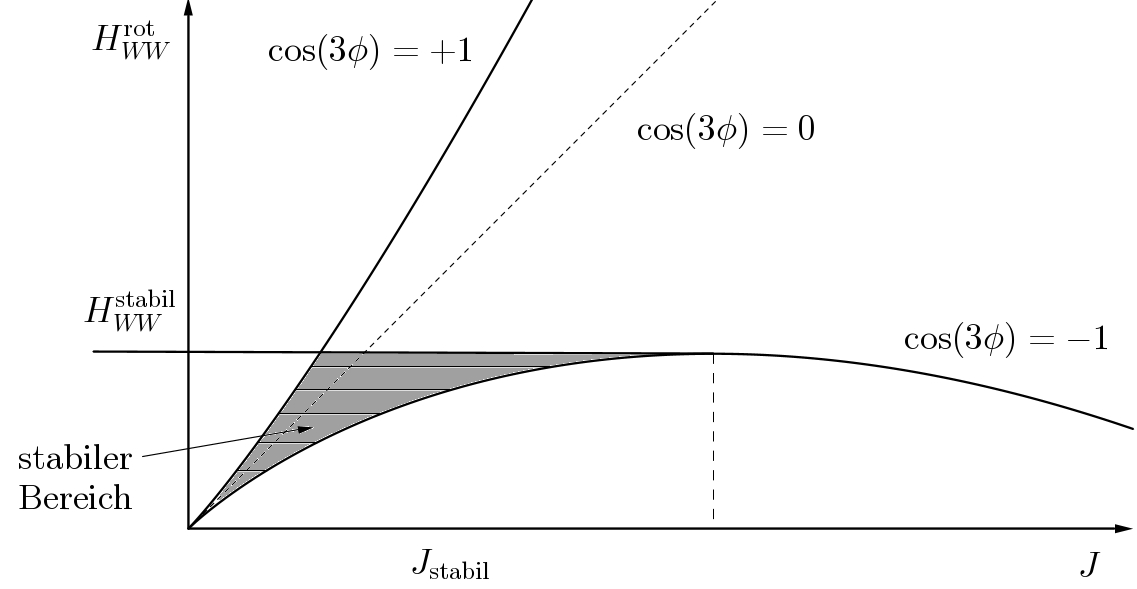
\includegraphics[width=1\textwidth]{../pics/Hstabil.jpg}
\end{figure} 
\end{frame}

\begin{frame}
 \frametitle{Verhalten in Resonanznähe}
 \pause
 In stabilem Bereich gibt es für kleine $H_{WW}^\text{rot}$ immer ein passendes $J$, unabhängig von $\phi$. Dies gilt bis:
 \begin{align*}
  (J_\text{stabil},\,H_{WW}^\text{stabil}) = \left(32\left(\frac{\delta Q}{\sqrt{C^2+D^2}}\right)^2,\, \frac{32}{3R}\frac{(\delta Q)^3}{C^2+D^2}\right)
 \end{align*}

\end{frame}

\begin{frame}
 \frametitle{Fixpunkte}
 \pause
 Fixpunkte ändern sich nicht mit $s$:
 \begin{align*}
  \frac{\partial H_{WW}^\text{rot}}{\partial J} &= A + \frac32 BJ^{1/2}\cos(3\phi_\text{rot} + \phi_0) = 0\\
  -\frac{\partial H_{WW}^\text{rot}}{\partial \phi_\text{rot}} &= \sin(3\phi_\text{rot} + \phi_0) = 0\\
  &\rightarrow \phi_\text{rot} = -\frac{\phi_0}{3}+\left(0,\frac{\pi}{3}, \frac{2\pi}{3}, \pi, \frac{4\pi}{3}, \frac{5\pi}{3}\right)\\
  &\rightarrow \cos(3\phi_\text{rot} + \phi_0) = \pm 1 \quad(\text{abh. A,B-VZ})
 \end{align*}
 

\end{frame}

\section{Ausblick}
\begin{frame}
 \frametitle{Oktupol}
 \pause
 Hamiltonfunktion mit Oktupolpotenzial $A_s = C(2J\beta)^2 \cos(\phi)^4$:
 \begin{align*}
  H_{WW} = \frac{J}{\beta}+ \frac{C}{2}\beta^2J^2(\cos(4\phi)+4\cos(2\phi)+3)
 \end{align*}
 Betatronphasenvorschub:
 \begin{align*}
  \frac{\partial H_{WW}}{\partial J }= \frac{1}{\beta} + C \beta^2J(\underbrace{\cos(4\phi)}_{\text{Res 4.Ord}}+4\cos(2\phi)+\underbrace{3}_{\text{Tune shift}})
 \end{align*}
Die Hälfte der Fixpunkte des Oktupols sind instabil, zeichnen sich also durch Bifurkation der Trajektorie aus.
 
\end{frame}


\begin{frame}
 \frametitle{Kopplung}
 \pause
 \begin{itemize}
  \item Bisher $y=0$
  \item $c\cdot y^n$ im Vektorpotential sind analog zu horizontalen Komponente 
  \item $x^n\cdot y^m$ führen zu Kopplung
  \item[$\rightarrow$] mehrdimensionale Beschreibung notwendig (Erhaltungssätze gelten oft bis 4 Dimensionen)
 \end{itemize}

\end{frame}

\begin{frame}
 \frametitle{Gegenwart vieler Nichtlinearitäten}
 \begin{itemize}
  \item Bei Nichtlinearitäten mit $x^n\cdot y^m$ alle $Q_x/Q_y$ resonant mit $nQ_x + mQ_y = p$
  \item Resonanzen bis 10. Ordnung bei $p$-Ringen, 4. Ordnung bei $e^-$-Ringen
  \item isolierte Resonanzen sind deterministisch
  \item Chirikov-Kriterium für chaotisches Verhalten vieler Resonanzen
 \end{itemize}

 
\end{frame}




\end{document}




\section{Transformation auf Wirkungs-Winkel-Variable}
\subsection{Bedeutng der Wirkungs-Winkel-Variablen}
\begin{frame}
 \frametitle{Bedeutende Größen}
\end{frame}

\subsection{Beispiele}
\begin{frame}
 \frametitle{Beispiel: Gradientenfehler}
\end{frame}

\begin{frame}
 \frametitle{Beispiel: Sextupol}
\end{frame}

\section{Resonanzen}
\begin{frame}
 \frametitle{Beispiel: Sextupol}
\end{frame}

\begin{frame}
 \frametitle{Verhalten in Resonanznähe}
\end{frame}

\begin{frame}
 \frametitle{Fixpunkte}
\end{frame}

\section{Ausblick}
\begin{frame}
 \frametitle{Oktupol}
\end{frame}

\begin{frame}
 \frametitle{Kopplung}
\end{frame}

\begin{frame}
 \frametitle{Gegenwart vieler Nichtlinearitäten}
\end{frame}




\end{document}